\documentclass{ezb}
\usepackage[]{todonotes}
\usepackage{amsmath}
\usepackage{gensymb}
\usepackage{wrapfig}
\usepackage{longtable}
\usepackage{amssymb}
\usepackage[colorlinks,        	% Links ohne Umrandungen in zu wählender Farbe
   linkcolor=black,   			% Farbe interner Verweise
   filecolor=black,   			% Farbe externer Verweise
   citecolor=black    			% Farbe von Zitaten
]{hyperref}
\usepackage{booktabs}

\renewcommand{\thesubsection}{\alph{subsection}}
\begin{document}

% \maketitle{Nummer}{Abgabedatum}{Tutor-Name}{Gruppennummer}
%           {Teilnehmer 1}{Teilnehmer 2}{Teilnehmer 3}
\maketitle{05.06.15}{Udo Frese}{1}{Annika Ofenloch - 2992807 - ofenloch@uni-bremen.de}{Frank Ihle - 3010158 - fihle@uni-bremen.de}{Simon Schirrmacher - 4000884 - simons@informatik.uni-bremen.de}{Noshaba Cheema - ncheema@uni-bremen.de}

%-------Text-Start------------------------------------------
\section{Ballspiele II}
\newpage
\section{Freistoß (4 Punkte)}
Bei einer Fußball-TV-Übertragung soll für den Zuschauer die Zone in das Bild eingezeichnet werden, auf der sich kein Gegenspieler bei einem Freistoß befinden darf.
\subsection{Allgemein}
Der Algorithmus orientiert sich an bekannten Objekten, deren Dimensionen im physikalischen Raum ihm bekannt sind. Die meisten Bemaßungen auf einem Fußballfeld sind festgeschrieben und falls es hiervon Abweichungen gibt, können diese vor Spielbeginn eingeholt und händisch eingetragen werden.\\
\linebreak
Das Fußballfeld ist rechteckig, aber je nach Blickwinkel der Kamera ergeben sich Bildverzerrungen (beispielsweise erscheint der Platz, wenn die Kamera flach, von der Seite sowie mittig auf das Spielfeld schaut, trapezförmig). Diese Verzerrung muss ebenso beim Kreis berücksichtigt werden. So wird aus dem Kreis eine Ellipse, deren kurze Diagonale umso größer wird, je näher die Ellipse an der Kamera ist. Diese Verzerrung kann durch die Kameragleichung ermittelt werden (siehe Gleichung \ref{eq:Kameragleichung})\\
\linebreak
Wenn nun bekannt ist, mit welchen Parametern die Ellipse eingezeichnet werden soll, gibt es hierfür zwei Möglichkeiten. Zum einen kann statisch festlegen werden, dass das Kamerabild genau an einer Stelle stehen bleibt und erst beim Anspielen wieder geschwenkt werden darf, da sich ab hier der Kreis wieder auflösen soll - so muss die Zone nur einmal berechnet und eingetragen werden. Für die nachfolgenden Bilder
kann diese dann einfach rein kopiert werden. \\
\linebreak
\todo[inline]{
	- die nachfolgenden Bilder, die von der gleichen Perspektive aufgenommen werden? Oder welche Bilder meinst du damit?}
Die andere Möglichkeit besteht darin, den Freistoß-Kreis beim Zoom-Vorgang zu zeigen. Hierfür werden mindestens zwei Bilder benötigt, auf denen Objekte zu sehen sind, deren reale Größe bekannt sind (siehe \ref{b:skaliergr} Skaliergrößen). Im Mittelpunkt der Bilder ist der Ball und es werden wie gewohnt die Ellipsen berechnet. Da sich aber beim Zoomen die Zone im Folgebild vergrößert, kann nun ein $\vartriangle r$ berechnet werden und für die nächsten Aufnahmen (vor allem für diese, wo kein Objekt mit bekannter Größe zu erkennen ist) der Radius und dadurch die Ellipse definiert werden. Da dies einer linearen Zoom-Funktion entspricht, funktioniert dieses Verfahren ausschließlich bei konstanter Vergrößerungsgeschwindigkeit. Wenn mehr als zwei Aufnahmen zur Berechnung von $\vartriangle r$ verwendet und deren Ergebnis gemittelt werden, lässt sich dieser Faktor genauer einstellen.
\subsection{Skaliergrößen}\label{b:skaliergr}
Nachfolgend, Beispiele für Objekte mit bekannten Ausmaßen, mit deren Hilfe letztlich die Freistoßzone definiert werden kann: Torlatte und -pfosten, Rasenmuster sowie die weiße Linien (darunter: Seiten- und Mittellinien, Strafraum und Anstoßkreis). 
\subsection{Kameraeinstellung}
Ein Bildpunkt im Weltkoordinatensystem kann auf das Kamerasystem mit nachfolgender Gleichung umgerechnet werden:\\
\begin{small}
\begin{equation}
\left(
\begin{array}{c}
      u \\
      v
\end{array}
\right)
=
\left(
\begin{array}{c}
      u_{0} \\
      v_{0}
\end{array}   
\right)
+ \alpha \cdot d_{\kappa1 ,\kappa2}(p(T^{-1}_{W\leftarrow C}\cdot p^{W})) 
\label{eq:Kameragleichung}
\end{equation}
\end{small}
Die Transformationsmatrix wird mit der nachfolgenden Gleichung \ref{eq:Transformationsmatrix} beschrieben.\\
\begin{small}
\begin{equation}
\textbf{T}_{W\leftarrow B}=
\begin{pmatrix}
1 & &  & x_{Ball} \\
 & 1 & & y_{Ball} \\
 & & 1 & z_{Ball} \\
 & & & 1
\end{pmatrix}
\cdot
\begin{pmatrix}
1 & &  & \\
 & cos \alpha_{r} & -sin \alpha_{r} & \\
 & sin \alpha_{r} & cos \alpha_{r} & \\
 & & & 1
\end{pmatrix}
\cdot
\begin{pmatrix}
cos \beta_{r} & & sin \beta_{r} & \\
 & 1 & & \\
-sin \beta_{r} & & cos \beta_{r} & \\
 & & & 1
\end{pmatrix}
\cdot
\begin{pmatrix}
cos \gamma_{r} & -sin \gamma_{r} & & \\
sin \gamma_{r} & cos \gamma_{r} & & \\
 & & 1 & \\
 & & & 1
\end{pmatrix}
\label{eq:Transformationsmatrix}
\end{equation}  
\end{small}
\linebreak
Hier sind $\alpha_{r}, \beta_{r}, \gamma_{r}$ die Winkel zwischen dem ursprünglichen und dem um jeweils die drei Achsen verdrehten Koordinatenkreuz, die allerdings variabel sind. Repräsentativ für die anderen Winkel soll die Winkelberechnung anhand der Beziehung für $\alpha_{r}$ erläutert werden, die in Abb. \ref{abb:alpharBerechnung} veranschaulicht ist.\\
\linebreak
Die blaue Strecke teilt das Feld in zwei Bereiche auf, sie ist gleichzeitig die Spiegelachse für $alpha_{r}$ und orientiert sich an der Kameraposition (hier ist $x=0$). So haben Strecken, die parallel zur Torlinie verlaufen, aus dieser Perspektive in der linken Hälfte eine positive Steigung und in der rechten eine negative Steigung. Aus diesem Grund muss hier auch eine Fallunterscheidung gemacht werden, sodass $\alpha_{r}$ immer über das Winkel/Positionsverhältnis berechnet, wie in Gleichung \ref{eq:alphar} beschrieben. Eine Ähnliche Berechnung muss für die beiden anderen Verdrehungswinkel des Koordinatenkreuzes durchgeführt werden ($ \beta , \gamma$) 
\todo[inline]{
-Per Schaubild verdeutlichen wieso man alle winkel braucht.\\
-dk1k2 ausformelieren ?
}.
\begin{equation}
\alpha_{r} = 
\begin{cases}
	\frac{\pi}{2} - (\frac{\pi}{2}-\alpha_{1,min}\frac{b'}{x}) & wenn \ x\geq 0  \\
    \frac{\pi}{2} - (\frac{\pi}{2}-\alpha_{2,min}\frac{b-b'}{x}) & wenn \ x\leq 0 \\
\end{cases}
\label{eq:alphar}
\end{equation}
\begin{figure}[!h]
\centering
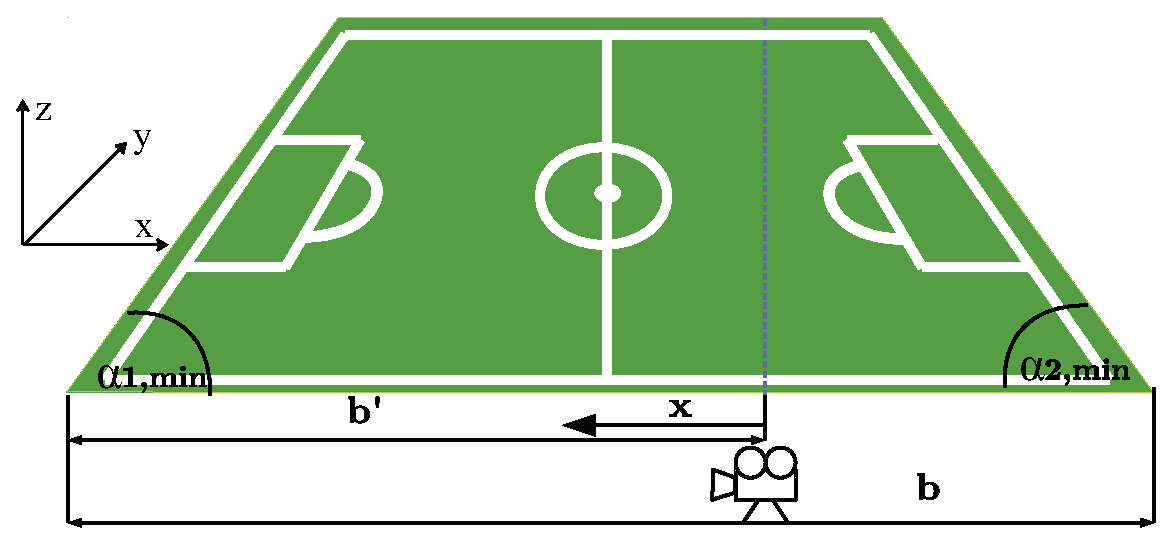
\includegraphics[scale=0.6]{./ar.eps}
\caption{Veranschaulichung für die $\alpha_{r}$-Berechnung}
\label{abb:alpharBerechnung}
\end{figure}
\subsection{Beurteilung}
Da beim Fußball schon wenige cm entscheidend sind, sollte der einzusetzende Algorithmus genaue Ergebnisse liefern, da \glqq Fehlentscheidungen\grqq \ ansonsten den Zuschauer verärgern können. Die unter diesen Bedingungen, gezeigten Methoden haben vermutlich nur eine begrenzte Genauigkeit, je nachdem wie exakt ein Objekt mit bekannter Größe erfasst wird (Negativbeispiel: Auflösung des Fußballs bei Aufnahme aus der Entfernung).
\section{Der einäugige Ballfangkönig (1 Punkt)}
Um den Skalenmaßstab aus den Messungen zu bestimmen, soll eine Analyse der Situation durchgeführt werden. Zum einen lässt sich der Skalenmaßstab über die Tiefenschärfe und zum anderen über die Flugbahn des Balls ermitteln. Bei der Flugbahn werden zwei Ansätze betrachtet. Im Folgenden werden die drei Verfahren kurz erläutert.
% Tiefenschärfe-Verfahren (Kamera-Parameter)
\subsection{Verfahren mit Hilfe der Tiefenschärfe}
Die Brennweite bestimmt den Abstand Linsenhauptebene und ihrem Brennpunkt. Ist nun also diese Brennweite (Abstand in z.B.: Metern) bei einer Kamera gegeben, so kennt man den Abstand eines Objekts zur Linse, wenn dieses den höchsten Schärfegrad erreicht hat. Dies kann beispielhaft bei unserem Ballwurfszenario implementiert werden. Hier wird einfach für jedes Bild die Kantenbreite über Sobel berechnet und das Bild mit der schmalsten Ballkante, ist dann dem Fokus der Kameralinse am nächsten. Die Genauigkeit der Methode hängt zum einen von der Genauigkeit der Brennweitenangabe und zum anderen von der Möglichkeit, den Ball genau im Brennpunkt erfassen zu können, ab.\\
\linebreak
Der Balldurchmesser kann demnach mit Hilfe der internen Kamerabemaßungen und dem Strahlensatz ermitteln werden. Wenn $\overline{AB}$ die Breite des Fotochips, $\overline{A'B'}$ die Breite des sich auf der Linse befindenden Bilds, $\overline{A''B''}$ der Balldurchmesser, $d_{1}$ der Abstand vom Fotochip zur Linsenhauptebene und $d_{2}$ die Brennweite ist, kann $\overline{A''B''}$  wie folgt berechnet werden (siehe. Abb \ref{abb:Strahlensatz}):\\
\linebreak
\begin{figure}[!h]
\centering
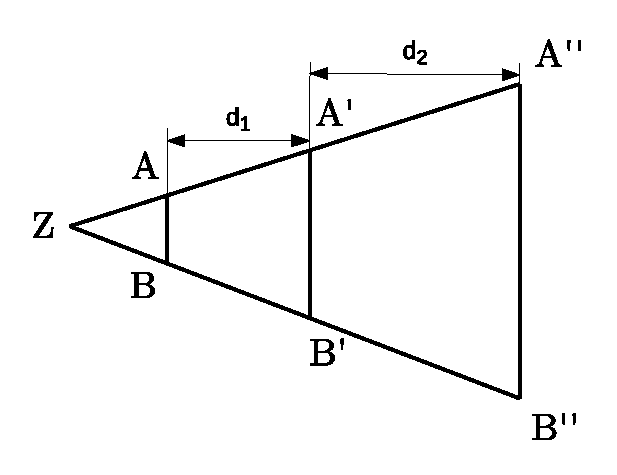
\includegraphics[scale=0.6]{./Strahlensatz.eps}
\caption{Veranschaulichung für die Balldurchmesserberechnung mit Hilfe der Tiefenschärfe.}
\label{abb:Strahlensatz}
\end{figure}
\begin{center}
$\frac{\overline{AB}}{\overline{A'B'}} = \frac{\overline{ZA}}{\overline{ZA'}} = \frac{\overline{ZA}}{\overline{ZA}+\overline{AA'}}$\\
$(\overline{ZA}+\overline{AA'})\frac{\overline{AB}}{\overline{A'B'}}-\overline{ZA}=0$\\
$\overline{ZA}=\frac{\overline{AA'}\frac{AB}{A'B'}}{1-\frac{AB}{A'B'}}$
\end{center}
mit
\begin{center}
$\overline{A'A} = \sqrt{d_{1}^{2}+(\frac{\overline{A'B'}}{2}-\frac{\overline{AB}}{{2}})^{2}}$\\
\end{center}
dann erhält man über
\begin{center}
$\frac{\overline{AB}}{\overline{A''B''}} = \frac{\overline{ZA}}{\overline{ZA''}} = \frac{\overline{ZA}}{\overline{ZA}+\overline{AA'}+\overline{A'A''}} $\\
\end{center}
mit
\begin{center}
$\overline{A'A''} = \sqrt{d_{2}^{2}+(\frac{\overline{A''B''}}{2}-\frac{\overline{A'B'}}{{2}})^{2}}$\\
\end{center}
das gesuchte $\overline{A''B''}$ mit folgender Berechnung:\\
\begin{center}
$\overline{A''B''} = \frac{\overline{ZA}+\overline{AA'}+\overline{A'A''}}{\overline{ZA}}\overline{AB}$
\end{center}
\subsection{Verfahren mit Hilfe der Ballflugbahn}
% Bahngleichung
\subsubsection*{Erster Ansatz}
Des Weiteren lässt sich der Skalenmaßstab über die Flugbahn des Balls berechnen, welche aus den vorhandenen Messungen hervorgeht. Es handelt sich hierbei um einen schrägen Wurf.
Die Aufnahmezeit der einzelnen Frames ist bekannt, sodass über den Wurfwinkel $\alpha$ die Anfangsgeschwindigkeit $v_0$ ermittelt werden kann, wenn angenommen wird, dass die Ballposition auf dem ersten Frame den Start repräsentiert. $v_0$ setzt sich aus den Komponenten $v_x$ und $v_y$ zusammen und ist Abhängigkeit vom Abwurfwinkel $\alpha$ (siehe Abbildung \ref{abb:geschwindigkeiten}). $v_y$ stellt hierbei die Geschwindigkeit in y-Richtung und $v_x$ die Geschwindigkeit in x-Richtung dar und lassen sich über die folgenden Gleichungen ausdrücken:
\begin{center}
$v_x = v_0 * cos(\alpha)$ \\
$v_y = v_0 * sin(\alpha)$
\end{center}
\begin{figure}[!h]
	\centering
	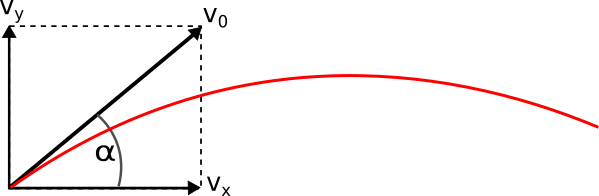
\includegraphics[scale=0.8]{./img/geschwindigkeitsrichtung.png}
	\caption{Geschwindigkeitsvektoren $v_0$, $v_x$ sowie $v_y$}
	\label{abb:geschwindigkeiten}
\end{figure}
Mittels des Geschwindigkeit-Zeit-Gesetzes, wo ebenso die Erdbeschleunigung ($g = 9.81m/s^2$) und Steigzeit $t_H$ einbezogen wird, lässt sich die Geschwindigkeit $v_y$ bei einem schrägen Wurf wie folgt berechnen:
\begin{center}
$v_y = v_0 * sin(\alpha) - g * t_H$
\end{center}
Da $v_y$ am höchsten Punkt der Bahnkurve gleich 0 ist, lässt sich die Gleichung nach $v_0$ umstellen. Bei $t_H$ handelt es sich um die vergangene Zeit vom ersten Bild (Start bei $t_1$) bis zum Bild mit dem höchsten Punkt der Bahnkurve (Maximum bei $t_2$), wie in Abbildung \ref{abb:ballflugbahn} zu sehen ist. Da alle Parameter bekannt sind, kann die Anfangsgeschwindigkeit $v_0$  mit der Gleichung 
\begin{center}
	$v_0 = \dfrac{g * t_H}{sin(\alpha)}$
\end{center}
berechnet werden.
\begin{figure}[!h]
	\centering
	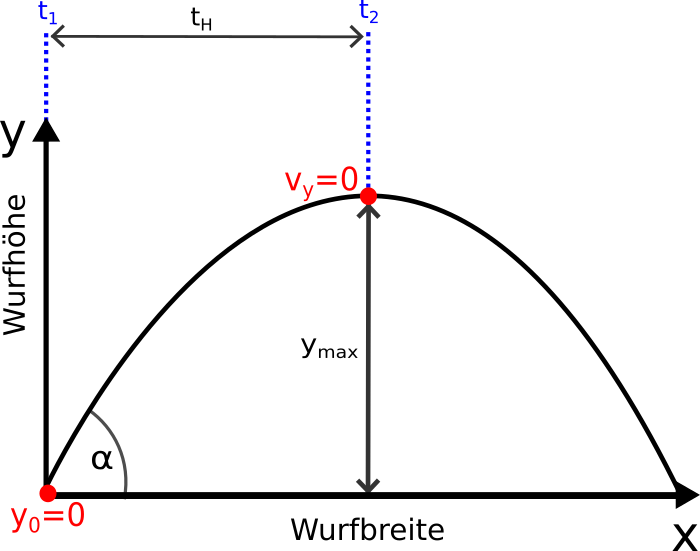
\includegraphics[scale=1.5]{./img/BallflugbahnAnsatz1.png}
	\caption{Ballflugbahn}
	\label{abb:ballflugbahn}
\end{figure}
Anschließend kann die maximale Wurfhöhe $y_{max}$ unter Verwendung des Ort-Zeit-Gesetz über die nachfolgende Gleichung ermittelt werden, wobei $y_0$ gleich 0 ist:
\begin{center}
$y_{max} = y_0 + v_0 * sin(\alpha) * t_H - g * (t_{H})^{2}$
\end{center}
Wenn nun die Länge der maximalen Ballhöhe, wie in Abbildung \ref{abb:ballflugbahn} zu sehen ist, bekannt ist, verfügt man über einen Skalenmaßstab mit dem zum Beispiel der Balldurchmesser bestimmt werden kann. Es handelt sich hierbei jedoch nur um eine Approximation, da die z-Richtung des Wurfes nicht mit einbezogen wurde. 

Für ein genaueres Ergebnis könnte die Tiefeninformation über den zuvor beschriebenen Tiefenschärfe-Ansatz einbezogen werden, sodass beide Verfahren kombiniert werden.
\todo[inline]{Kann man das so schreiben? Oder sollten wir das lieber weglassen mit der kombinierten Variante, da wir die ja nicht weiter erläutern werden?}

\subsubsection*{Zweiter Ansatz}
Das zweite Verfahren zur Bestimmung des Skalenmaßstabs über die Ballflugbahn macht sich das Unabhängigkeitsgesetz zu nutze. Der Ball bewegt sich von der maximalen Wurfhöhe zum Zeitpunkt $t_2$ aus kurvenförmig zum Boden hin. Wenn ein weiterer Ball von der maximalen Höhe zum Zeitpunkt $t_2$ im freien Fall nach unten fallen würde, würden beide Bälle den Boden zum selben Zeitpunkt erreichen. Dieses Phänomen machen wir uns zu nutze, indem wir die Strecke $h$ für den freien Fall ermitteln, also die Entfernung von der maximalen Wurfhöhe bis zum Aufprall (siehe Abbildung \ref{abb:freierfall}). Diese Strecke $h$ wird mittels folgender Gleichung berechnet:
\begin{center}
$h = \dfrac{g * (t_H)^2}{2}$
\end{center}
\begin{figure}[!h]
	\centering
	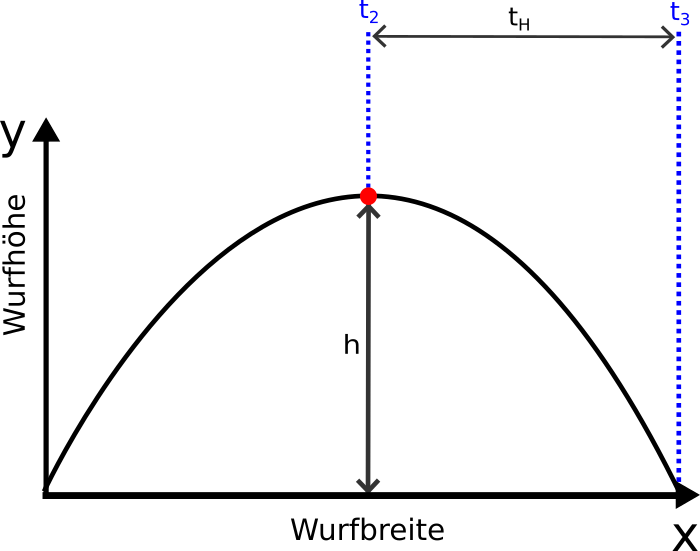
\includegraphics[scale=1.5]{./img/BallflugbahnAnsatz2.png}
	\caption{Ballflugbahn}
	\label{abb:freierfall}
\end{figure}
$t_H$ ist in diesem Fall die Fallzeit von $t_2$ bis zum Aufprall auf dem Boden. Aufgrund des Unabhängigkeitsgesetzes ist die Fallzeit über die Bildaufnahmen bekannt.
Diese Strecke $h$ stellt ebenso einen Skalenmaßstab im Bild dar, wodurch unter anderem der Balldurchmesser ermittelt werden kann. Auch bei diesem Verfahren handelt es sich nur um eine Approximation, da die z-Richtung des Wurfes nicht mit einbezogen wird. Das Ergebnis reicht jedoch für unseren Anwendungsfall aus.
\todo[inline]{Kann man dazu Approximation sagen o.O?}
Hinzu kommt, dass bei den Berechnungen angenommen wurde, dass kein Luftwiderstand vorhanden ist (Annahme erfolgte ebenso bei der Programmieraufgabe).




%-------Text-End------------------------------------------
\end{document}

